% Options for packages loaded elsewhere
\PassOptionsToPackage{unicode}{hyperref}
\PassOptionsToPackage{hyphens}{url}
\PassOptionsToPackage{dvipsnames,svgnames,x11names}{xcolor}
%
\documentclass[
  10pt,
  a4paper,
]{scrreprt}

\usepackage{amsmath,amssymb}
\usepackage{iftex}
\ifPDFTeX
  \usepackage[T1]{fontenc}
  \usepackage[utf8]{inputenc}
  \usepackage{textcomp} % provide euro and other symbols
\else % if luatex or xetex
  \usepackage{unicode-math}
  \defaultfontfeatures{Scale=MatchLowercase}
  \defaultfontfeatures[\rmfamily]{Ligatures=TeX,Scale=1}
\fi
\usepackage{lmodern}
\ifPDFTeX\else  
    % xetex/luatex font selection
\fi
% Use upquote if available, for straight quotes in verbatim environments
\IfFileExists{upquote.sty}{\usepackage{upquote}}{}
\IfFileExists{microtype.sty}{% use microtype if available
  \usepackage[]{microtype}
  \UseMicrotypeSet[protrusion]{basicmath} % disable protrusion for tt fonts
}{}
\makeatletter
\@ifundefined{KOMAClassName}{% if non-KOMA class
  \IfFileExists{parskip.sty}{%
    \usepackage{parskip}
  }{% else
    \setlength{\parindent}{0pt}
    \setlength{\parskip}{6pt plus 2pt minus 1pt}}
}{% if KOMA class
  \KOMAoptions{parskip=half}}
\makeatother
\usepackage{xcolor}
\usepackage[inner=2cm,outer=2cm,top=2cm,bottom=2cm,headsep=22pt,headheight=11pt,footskip=33pt,ignorehead,ignorefoot,heightrounded]{geometry}
\setlength{\emergencystretch}{3em} % prevent overfull lines
\setcounter{secnumdepth}{1}
% Make \paragraph and \subparagraph free-standing
\ifx\paragraph\undefined\else
  \let\oldparagraph\paragraph
  \renewcommand{\paragraph}[1]{\oldparagraph{#1}\mbox{}}
\fi
\ifx\subparagraph\undefined\else
  \let\oldsubparagraph\subparagraph
  \renewcommand{\subparagraph}[1]{\oldsubparagraph{#1}\mbox{}}
\fi


\providecommand{\tightlist}{%
  \setlength{\itemsep}{0pt}\setlength{\parskip}{0pt}}\usepackage{longtable,booktabs,array}
\usepackage{calc} % for calculating minipage widths
% Correct order of tables after \paragraph or \subparagraph
\usepackage{etoolbox}
\makeatletter
\patchcmd\longtable{\par}{\if@noskipsec\mbox{}\fi\par}{}{}
\makeatother
% Allow footnotes in longtable head/foot
\IfFileExists{footnotehyper.sty}{\usepackage{footnotehyper}}{\usepackage{footnote}}
\makesavenoteenv{longtable}
\usepackage{graphicx}
\makeatletter
\def\maxwidth{\ifdim\Gin@nat@width>\linewidth\linewidth\else\Gin@nat@width\fi}
\def\maxheight{\ifdim\Gin@nat@height>\textheight\textheight\else\Gin@nat@height\fi}
\makeatother
% Scale images if necessary, so that they will not overflow the page
% margins by default, and it is still possible to overwrite the defaults
% using explicit options in \includegraphics[width, height, ...]{}
\setkeys{Gin}{width=\maxwidth,height=\maxheight,keepaspectratio}
% Set default figure placement to htbp
\makeatletter
\def\fps@figure{htbp}
\makeatother
\newlength{\cslhangindent}
\setlength{\cslhangindent}{1.5em}
\newlength{\csllabelwidth}
\setlength{\csllabelwidth}{3em}
\newlength{\cslentryspacingunit} % times entry-spacing
\setlength{\cslentryspacingunit}{\parskip}
\newenvironment{CSLReferences}[2] % #1 hanging-ident, #2 entry spacing
 {% don't indent paragraphs
  \setlength{\parindent}{0pt}
  % turn on hanging indent if param 1 is 1
  \ifodd #1
  \let\oldpar\par
  \def\par{\hangindent=\cslhangindent\oldpar}
  \fi
  % set entry spacing
  \setlength{\parskip}{#2\cslentryspacingunit}
 }%
 {}
\usepackage{calc}
\newcommand{\CSLBlock}[1]{#1\hfill\break}
\newcommand{\CSLLeftMargin}[1]{\parbox[t]{\csllabelwidth}{#1}}
\newcommand{\CSLRightInline}[1]{\parbox[t]{\linewidth - \csllabelwidth}{#1}\break}
\newcommand{\CSLIndent}[1]{\hspace{\cslhangindent}#1}

\addtokomafont{disposition}{\rmfamily}
\usepackage{ragged2e}
\usepackage{blindtext}\usepackage{amsthm}
\usepackage{amsthm}
\usepackage{hyperref}
\newtheorem{thm}{Theorem}[subsection]
\renewcommand{\thethm}{\arabic{subsection}.\arabic{thm}}

\makeatletter
\makeatother
\makeatletter
\makeatother
\makeatletter
\@ifpackageloaded{caption}{}{\usepackage{caption}}
\AtBeginDocument{%
\ifdefined\contentsname
  \renewcommand*\contentsname{Table of contents}
\else
  \newcommand\contentsname{Table of contents}
\fi
\ifdefined\listfigurename
  \renewcommand*\listfigurename{List of Figures}
\else
  \newcommand\listfigurename{List of Figures}
\fi
\ifdefined\listtablename
  \renewcommand*\listtablename{List of Tables}
\else
  \newcommand\listtablename{List of Tables}
\fi
\ifdefined\figurename
  \renewcommand*\figurename{Figure}
\else
  \newcommand\figurename{Figure}
\fi
\ifdefined\tablename
  \renewcommand*\tablename{Table}
\else
  \newcommand\tablename{Table}
\fi
}
\@ifpackageloaded{float}{}{\usepackage{float}}
\floatstyle{ruled}
\@ifundefined{c@chapter}{\newfloat{codelisting}{h}{lop}}{\newfloat{codelisting}{h}{lop}[chapter]}
\floatname{codelisting}{Listing}
\newcommand*\listoflistings{\listof{codelisting}{List of Listings}}
\usepackage{amsthm}
\theoremstyle{plain}
\newtheorem{conjecture}{Conjecture}[section]
\theoremstyle{definition}
\newtheorem{definition}{Definition}[section]
\theoremstyle{plain}
\newtheorem{theorem}{Theorem}[section]
\theoremstyle{remark}
\AtBeginDocument{\renewcommand*{\proofname}{Proof}}
\newtheorem*{remark}{Remark}
\newtheorem*{solution}{Solution}
\makeatother
\makeatletter
\@ifpackageloaded{caption}{}{\usepackage{caption}}
\@ifpackageloaded{subcaption}{}{\usepackage{subcaption}}
\makeatother
\makeatletter
\@ifpackageloaded{tcolorbox}{}{\usepackage[skins,breakable]{tcolorbox}}
\makeatother
\makeatletter
\@ifundefined{shadecolor}{\definecolor{shadecolor}{rgb}{.97, .97, .97}}
\makeatother
\makeatletter
\makeatother
\makeatletter
\makeatother
\ifLuaTeX
  \usepackage{selnolig}  % disable illegal ligatures
\fi
\IfFileExists{bookmark.sty}{\usepackage{bookmark}}{\usepackage{hyperref}}
\IfFileExists{xurl.sty}{\usepackage{xurl}}{} % add URL line breaks if available
\urlstyle{same} % disable monospaced font for URLs
\hypersetup{
  pdftitle={Annual Progress Review},
  pdfauthor={Thomas William Boughen},
  colorlinks=true,
  linkcolor={blue},
  filecolor={Maroon},
  citecolor={Blue},
  urlcolor={Blue},
  pdfcreator={LaTeX via pandoc}}

\title{Annual Progress Review}
\author{Thomas William Boughen}
\date{May 31, 2024}

\begin{document}
\cleardoublepage
\thispagestyle{empty}
{\centering
\hbox{}\vskip 0cm plus 1fill
{\Huge\bfseries Annual Progress Review \par}
\vspace{12ex}
{\Large\bfseries Thomas William Boughen \par}
\vspace{3ex}
\vskip 0cm plus 2fill
%{\bfseries\large Doctor of Philosophy \par}
\vspace{3ex}
{\bfseries\large May 31, 2024 \par}
\vspace{12ex}
{
\includegraphics[width=0.1\linewidth]{"imgs/University_of_Newcastle_Coat_of_Arms.png"}\par}
%
%
{\bfseries\large Newcastle University \par}
\vspace{3ex}
%
{\bfseries\large School of Mathematics, Statistics and Physics \par}
%
\vspace{12ex}
%{\small Submitted in total fulfilment of the requirements
%of the degree of Doctor of Philosophy \par}
%}
\footnote{An html version of this report can be found at \url{www.twboughen.github.io/phd/APR/report}}
\justifying
\noindent\ifdefined\Shaded\renewenvironment{Shaded}{\begin{tcolorbox}[sharp corners, interior hidden, enhanced, borderline west={3pt}{0pt}{shadecolor}, boxrule=0pt, breakable, frame hidden]}{\end{tcolorbox}}\fi

\renewcommand*\contentsname{Table of contents}
{
\hypersetup{linkcolor=}
\setcounter{tocdepth}{1}
\tableofcontents
}
\hypertarget{sec-int}{%
\chapter{Introduction}\label{sec-int}}

Networks appear across appear in a range of fields of study including
but not limited to micro-biology, computer science, sociology, and
music. This makes them a valuable source of data to study, this report
will be focused on the processes by which these networks form. Often,
networks are assumed to have come from the Barabási-Albert model so that
a power law can be used to model their degree distribution however a
power law, while suitable for the bulk of the data, seems to become less
suitable for the most extreme values in the network.

Shown below in Figure~\ref{fig-survs1} are some examples of the degree
distribution of real networks along with some simulated from two network
generative processes given in Section~\ref{sec-gen}. The networks in
Figure~\ref{fig-survs1} are:

\begin{itemize}
\tightlist
\item
  \textbf{as-caida}: the undirected network of autonomous systems of the
  Internet connected with each other from the CAIDA project, collected
  in 2007. {[}\protect\hyperlink{ref-caida}{1}{]}
\item
  \textbf{BA simulated}: a network simulated using the Barabási-Albert
  model with \(m=1\) from Section~\ref{sec-gen}
\item
  \textbf{Jazz}: the collaboration network between Jazz musicians
  collected in 2003 {[}\protect\hyperlink{ref-jazz}{2}{]}
\item
  \textbf{Meta}: this is the metabolic network of the roundworm
  \emph{Caenorhabditis elegans} {[}\protect\hyperlink{ref-meta}{3}{]}
\item
  \textbf{Pajek-erdos}: This network contains people who have, directly
  and indirectly, written papers with Paul Erdős as of 2003.
  {[}\protect\hyperlink{ref-pajek}{4}{]}
\item
  \textbf{Reactome}: This is a network of protein--protein interactions
  in humans. {[}\protect\hyperlink{ref-reactome}{5}{]}
\item
  \textbf{UA simulated}: a network simulated using the uniform
  attachment model with \(m=1\) from Section~\ref{sec-gen}.
\end{itemize}

\begin{figure}[H]

{\centering 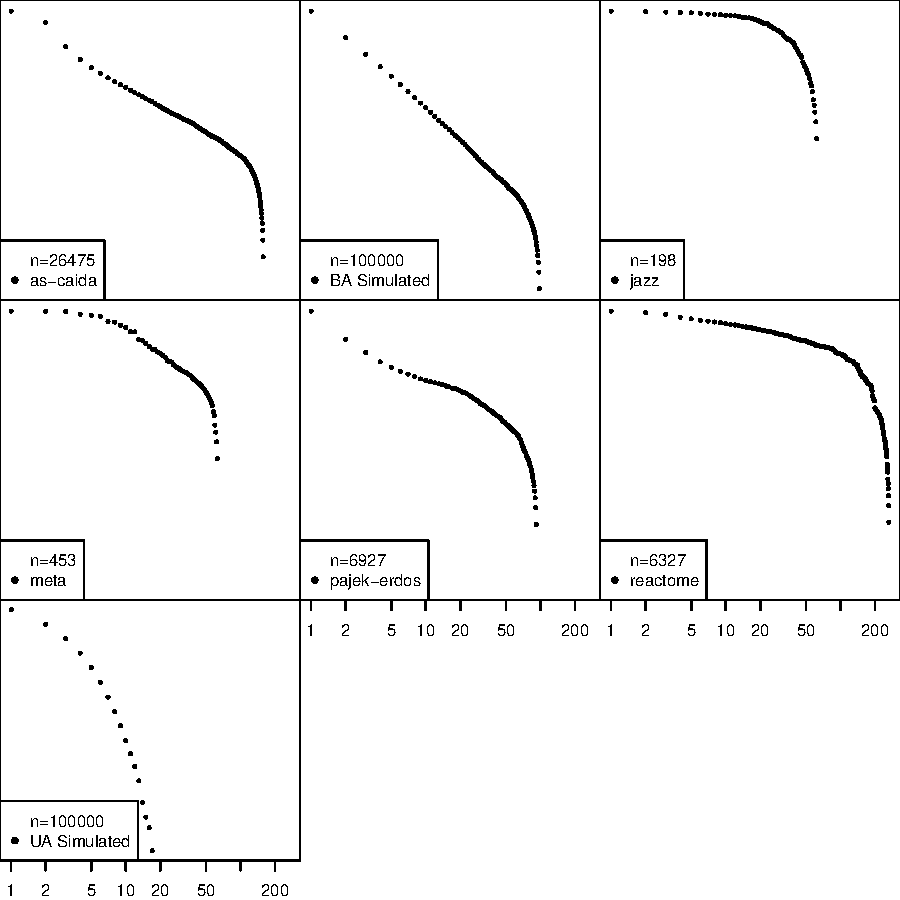
\includegraphics[width=0.66\textwidth,height=\textheight]{doc_files/figure-pdf/fig-survs1-1.pdf}

}

\caption{\label{fig-survs1}Plots of survival functions of real networks
degrees, along with the degree distribution for the UA and the BA
models}

\end{figure}

This report beings with a brief introduction to univariate extreme value
theory first for continuous values before moving to considerations for
discrete data. Following this, an introduction to networks, network
generative processes and some theoretical results for the networks that
arise from them.

Since the aim is to gain understanding about the behaviour of the degree
distribution of networks at the most extreme values, it seems natural to
look to using methods from extreme value theory.

\hypertarget{sec-ext}{%
\chapter{Univariate Extreme Value Theory}\label{sec-ext}}

This section begins with a review of the theory and methodology for
modelling the extreme values of continuous random variables, before
moving to considerations for modelling the extreme values of discrete
random variables.

\hypertarget{sec-ce}{%
\section{Continuous Extremes}\label{sec-ce}}

This section is a concise introduction to the two main methods for
modelling extreme values: block maxima and peaks over threshold

The first method considers the distribution of block maxima. That is,
for a set of independent and identically distributed (iid) random
variables \(X_1,\ldots,X_n\) with common cumulative density function
(cdf) \(F\), the block maxima approach studies the limiting distribution
of \(M_n = \max\{X_1,\ldots,X_n\}\).

Clearly, as \(n\rightarrow \infty\), the block maxima \(M_n\) converges
almost surely to the right endpoint of \(F\). However, standardising the
block maxima allows for some characterisation of the limiting
distribution. The following theorem is a key result in extreme value
theory as it derives the general form of all possible limit laws for the
standardised block maxima \(M_n*\). ::: \{\#thm-evt\}

\hypertarget{fishertippettgnedenko-theorem}{%
\subsection{Fisher--Tippett--Gnedenko
Theorem}\label{fishertippettgnedenko-theorem}}

With \(X_1, \ldots,X_n \overset{\mathrm{iid}}{\sim} F\) and
\(\{ a_n\}_{n\ge0}, \{ b_n\}_{n\ge0}\) such that:

\[\lim_{n\rightarrow\infty}\Pr\left[\displaystyle\frac{1}{a_n}\{M_n-b_n\}\le x\right] = G(x),\]
for some non-degenerate \(G\).

Then \(F\) is said to be in the (maximum) domain of attraction of \(G\),
denoted \(F\in\mathcal D(G)\) ,and \(G\) is of one of three types:

\begin{itemize}
\tightlist
\item
  Gumbel: \(\Lambda(x) = \exp\{-\exp(-x)\},\quad x \in \mathbb R\)
\item
  Fréchet:
  \(\Phi_\alpha(x) = \exp\{-x^{-\alpha}\},\quad x\ge 0,\alpha>0\)
\item
  Negative-Weibull:
  \(\Psi_\alpha(x) = \exp\{-x^{-a}\},\quad x<0,\alpha>0\)
\end{itemize}

See {[}\protect\hyperlink{ref-haan06}{6}{]} for the proof. :::

Each of these three types defines a domain of attraction.

\begin{definition}[Domains of
Attraction]\protect\hypertarget{def-doa}{}\label{def-doa}

The three domains of attraction that result from \textbf{?@thm-evt} have
the following equivalent conditions:

For a distribution with cdf \(F\) and survival function \(\bar F\) that
has right endpoint \(x_F\) given by: \[
x_F = \sup\{x \in \mathbb R \cup\{\infty\}:F(x)<1\}
\] the distribution belongs to each domain of attraction subject to the
conditions below:

\textbf{If there exists a positive function b}

\begin{itemize}
\tightlist
\item
  Type I/Gumbel/\(\mathcal D(\Lambda)\):
\end{itemize}

\[
\lim_{x\uparrow x_F} \displaystyle\frac{\bar F(x+tb(x))}{\bar F(x)} = e^{-t},\quad \forall t\in\mathbb R
\]

\textbf{If} \(x_F=\infty\):

\begin{itemize}
\tightlist
\item
  Type II/Fréchet/\(\mathcal D (\Phi_\alpha)\):
\end{itemize}

\[
\lim_{x\rightarrow\infty} \displaystyle\frac{\bar F(tx)}{\bar F(x)} = x^{-\alpha}, \quad \forall t>0 \quad \text{ for some } \alpha>0
\]

\textbf{If} \(x_F<\infty\):

\begin{itemize}
\tightlist
\item
  Type III/Negative-Weibull/\(\mathcal D(\Psi_\alpha)\):
\end{itemize}

\[
\lim_{h\downarrow 0}\displaystyle\frac{\bar F(x_F-xh)}{\bar F(x_F-h)} = x^\alpha, \quad\alpha>0
\]

\end{definition}

The parameter \(\alpha\) in Definition~\ref{def-doa} and
\textbf{?@thm-evt} is called the extreme value index.

Here, distributions in the Gumbel domain are referred to as light
tailed, distributions in the Negative-Weibull domain are referred to as
short tailed, and those in the Fréchet are referred to as heavy tailed.
This terminology for heavy tailed distributions is different to some of
the literature that defined a heavy tailed distribution as one that
decays slower than exponential. However the terminology used here is
also widely used.

Throughout this report functions will be referred to as regularly
varying or slowly varying, what is meant by this is formally defined
below:

\begin{definition}[Regular
Variation]\protect\hypertarget{def-rv}{}\label{def-rv}

A positive,real valued, measurable function \(f\) is said to be
regularly varying at infinity with index \(\gamma\) if for all \(t>0\):

\[
\lim_{x\rightarrow\infty}\displaystyle\frac{f(tx)}{f(x)} = x^{\gamma}.
\] If \(\gamma =0\), then \(f\) is instead said to be slowly varying at
infinity.

\end{definition}

Note that the condition for a distribution to belong to the Fréchet
domain of attraction is equivalent to saying that the survival function
\(\bar F\) is regularly varying with index \(-\alpha\).

In addition to heavy tailed distributions it is also useful to define
what will be referred to as super heavy tailed distributions. This term
is often just refers to specific distributions such as the log-Cauchy
,log-Gamma,and log-Weibull distributions but
{[}\protect\hyperlink{ref-fmh09}{7}{]} provides a more precise
definition below:

\begin{definition}[Super Heavy
Tails]\protect\hypertarget{def-sup}{}\label{def-sup}

A distribution is with survival function \(\bar F\) is said to have
super heavy tails if: \[
\lim_{x\rightarrow\infty}\displaystyle\frac{\bar F(tx)}{\bar F (x)} = 1,\qquad \forall t>0
\] That is, a distribution is called super heavy if its survival
function is slowly varying.

\end{definition}

The three main types of extremal distribution (Gumbel, Fréchet and
Negative-Weibull) can be united into one distribution, called the
Generalised Extreme Value (GEV) distribution.

\begin{definition}[Generalised Extreme Value
Distribution]\protect\hypertarget{def-gev}{}\label{def-gev}

Denoted by \(\text{GEV}(\mu,\sigma,\xi)\) the distribution is
characterised by three parameters \(\mu \in \mathbb R\) the location,
\(\sigma\in \mathbb R^+\) the scale, and the shape \(\xi\in \mathbb R\).
It has support on \(\{x\in \mathbb R:1+\xi(x-\mu)/\sigma > 0\}\) and has
cdf given by:

\[
G(x) = \begin{cases}\exp\left[-\left\{1+\displaystyle\frac{\xi(x-\mu)}{\sigma}\right\}_+^{-1/\xi}\right],&\xi\ne0\\
\exp\left[-\exp\left\{-\displaystyle\frac{x-\mu}{\sigma}\right\}\right],&\xi=0.
\end{cases}
\]

\end{definition}

The three types of extremal distribution are obtained from changing the
shape parameter \(\xi\), which corresponds to \(1/\alpha\) in
\textbf{?@thm-evt}. This change is generally made so that the largest
\(\xi\) corresponds to heavier tails of the distribution. Specifically,
\(\xi<0\), \(\xi=0\), \(\xi>0\), correspond to the negative Weibull,
Gumbel and the Fréchet domains of attraction respectively.

The second method for modelling, is to consider observations above a
large threshold, like the limiting distribution of block maxima, the
limiting distribution of these extreme values can be characterised by
the generalised Pareto (GP) distribution.

\begin{definition}[Generalised Pareto
Distribution]\protect\hypertarget{def-gp}{}\label{def-gp}

Consider a random variable \(X\) with the same cdf \(F\) as in
\textbf{?@thm-evt}, the Generalised Pareto (GP) distribution can be
obtained by using the GEV distribution and conditional probability such
that for large enough threshold the GP distribution approximately
describes the conditional distribution of threshold exceedances. More
precisely, for sufficiently large threshold \(u\) and the change of
variable to \(Y=X-u\): \[
\Pr(Y\le y | Y>0) = H(y) = \begin{cases}
1-\left(1+\displaystyle\frac{\xi y}{\sigma}\right)^{-1/\xi},&y>0,\xi\ne 0 \\
1-\exp\left(-\displaystyle\frac{y}{\sigma}\right),&y>0,\xi = 0
\end{cases}
\]

\end{definition}

Since this distribution was obtained using a
\(\text{GEV}(\mu,\sigma^*,\xi)\) the shape parameter \(\xi\) is
identical in both distributions and the shape parameter \(\sigma\) is
defined such that \(\sigma = \sigma^* + \xi(u-\mu)\).

It is also possible to derive the result without using the GEV, as shown
in {[}REF{]}.

\hypertarget{sec-disc}{%
\section{Discrete Extremes}\label{sec-disc}}

A lot of Section~\ref{sec-ce} is appropriate only for continuous random
variables and some of the results may not hold in a discrete setting. In
particular, a continuous distribution \(F\) being in certain domain of
attraction may not necessarily imply that a discretisation of \(F\)
remains in that domain of attraction.

\begin{definition}[Discretisation]\protect\hypertarget{def-disc}{}\label{def-disc}

The discretisation of a distribution with cdf \(F\) is given by

\[F^*(n) = F(n) - F(n-1), \quad n   \in \mathbb Z\]

\end{definition}

{[}\protect\hyperlink{ref-shimura12}{8}{]} provides conditions for a
discretisation of a continuous distribution to belong to the same domain
of attraction. In particular the following theorem which corresponds to
Theorem 1 in {[}\protect\hyperlink{ref-shimura12}{8}{]}.

\begin{theorem}[Domain of attraction
consistency]\protect\hypertarget{thm-shimura1}{}\label{thm-shimura1}

~

\begin{enumerate}
\def\labelenumi{(\alph{enumi})}
\tightlist
\item
  Every discretisation of distribution in \(\mathcal D(\Phi_\alpha)\)
  remains in \(\mathcal D(\Phi_\alpha)\).
\item
  The discretisation of a distribution remains in
  \(\mathcal D(\Lambda)\) if and only if the original is in
  \(\mathcal D(\Lambda)\cap \mathcal L\).
\end{enumerate}

Where \(\mathcal L\) is the set of long-tailed distributions that have
the property: \[
\lim_{x\rightarrow \infty}\displaystyle\frac{\overline F(x+1)}{\overline F(x)} = 1   
\]

\end{theorem}

In addition {[}\protect\hyperlink{ref-shimura12}{8}{]} introduces a
quantity useful for determining the domain of a attraction that a
discrete distribution belongs to.

\begin{definition}[Omega
Function]\protect\hypertarget{def-omega}{}\label{def-omega}

For a distribution \(F\) with survival function \(\overline F\) and some
\(n\in\mathbb Z^+\) let:

\[
\Omega(F,n) = \left(\log\displaystyle\frac{\overline F (n+1)}{\overline F (n+2)}\right)^{-1} - \left(\log\displaystyle\frac{\overline F (n)}{\overline F (n+1)}\right)^{-1}
\]

\end{definition}

This quantity plays an important role in Section~\ref{sec-meth} when
determining the domain of attraction to which the degree distribution of
a network generative model belongs. In particular a discrete
distribution is recoverable to the Fréchet domain of attraction
\(\mathcal D(\Phi_\alpha)\) if: \[
\lim_{n\rightarrow\infty}\Omega(F,n) = \alpha^{-1}
\]

Applying ideas from Section~\ref{sec-ce} to modelling discrete random
variables has been approached from many different directions. What
follows is a overview of some of the approaches that have been taken but
will see use in this report.

{[}\protect\hyperlink{ref-hds24}{9}{]} note that using the GP
distribution as an approximation in a discrete setting leads to bias in
the likelihood function and can lead to it being inadequate for
modelling. They propose two other peaks over threshold methods that rely
on parametric families of discrete distributions. The first, what they
refer to as the discrete generalised Pareto approximation is based on an
extension of the discrete survival function. The second, the generalised
Zipf distribution is obtained from an extension of the probability mass
function. Both methods are motivated theoretically for modelling of a
large class of discrete distributions and are shown in the paper to
either match or outperform using the GP to model discrete data directly.

{[}\protect\hyperlink{ref-agn22}{10}{]} first introduce an extended GP
distribution, a continuous distribution that extends the idea of
obtaining GP values from a probability integral transform (PIT) of
\(U(0,1)\) draws and instead considers a PIT of draws from any
distribution on \((0,1)\) such as a beta distribution. This distribution
is then discretised into their discrete extended GP distribution.

\hypertarget{sec-mod}{%
\section{Modelling}\label{sec-mod}}

The results from Section~\ref{sec-ce} allow the GEV and GP to be fitted
to the block maxima and peaks over threshold respectively. An example of
where modelling the GEV may be useful are when modelling monthly high
temperatures, fitting the GEV to historic data of peak monthly
temperatures may allow for future prediction of these temperatures.
Fitting the GP may be useful in other scenarios such as modelling the
strength of solar flares.

Typically, when fitting the GP, a sufficiently high threshold needs to
be specified beforehand. {[}\protect\hyperlink{ref-coles2001}{11}{]}
provides some empirical methods for specifying the threshold, one
approach is to use a threshold stability plot that uses maximum
likelihood to estimate the parameters of the GP for a large range of
thresholds. The threshold can be chosen as the point across all of the
plots after which the values of the parameters seems stable. One
particular issue when fitting the GP to data, is that the likelihoods
cannot be compared for different thresholds as changing the threshold
changes the amount of data being used.

Another more recent approach shown by
{[}\protect\hyperlink{ref-mac2012}{12}{]}, uses a spliced threshold
mixture to model the threshold exceedances where one distribution is
assumed for the bulk of the data and the GP is used for those values
above the threshold. To model discrete extremes, the approaches proposed
in the literature are use a discretisation of the GP such as the one
given below:

\begin{definition}[Intergral Generalised Pareto Distribution
(IGP)]\protect\hypertarget{def-igp}{}\label{def-igp}

Consider a random variable \(X\) with cdf \(F\), and consider the random
variable \(Y=\lfloor X \rfloor\). From Definition~\ref{def-gp},
\(X|X>u \sim GP(\sigma, \xi)\) for some sufficiently large
\(u\in \mathbb R^+\) and it can be obtained that the distribution of
\(Y|Y>u\) has distribution defined below:

\[
\Pr(Y=y>Y>u) = \left(1+\displaystyle\frac{\xi(y+1-\lceil u\rceil)}{\sigma_0+\xi\lceil u\rceil}\right)_+^{-1/\xi}-\left(1+\displaystyle\frac{\xi(y-\lceil u\rceil)}{\sigma_0+\xi\lceil u\rceil}\right)_+^{-1/\xi}
\]

For \(y=\lceil u\rceil,\lceil u\rceil+1, \ldots\) and
\(\xi \in \mathbb R\) and \(u, \sigma_0 \in \mathbb R^+.\)

\end{definition}

A spliced mixture model is given below that uses a general discrete
distribution for the bulk of the data and the IGP above some threshold
\(v\).

\begin{definition}[IGP Spliced
Mixture]\protect\hypertarget{def-mixigp}{}\label{def-mixigp}

\[
f(y) = \begin{cases}
(1-\phi)g(x), & y=1,2,\ldots, v\\
\phi\left[\left(1+\displaystyle\frac{\xi(y+1-v)}{\sigma_0+\xi v}\right)_+^{-1/\xi}-\left(1+\displaystyle\frac{\xi(y-v)}{\sigma_0+\xi v}\right)_+^{-1/\xi}\right],&y=v+1, v+2,\ldots
\end{cases}
\] where \(g\) is the probability mass function of some discrete
distribution with support equal to \(\{1,2,\ldots,v\}\) and
\(\xi \in \mathbb R\) , \(\sigma_0 \in \mathbb R^+\) and
\(v\in\mathbb Z^+.\)

\end{definition}

\hypertarget{sec-net}{%
\chapter{Networks}\label{sec-net}}

Networks are the data sources that the results from
Section~\ref{sec-ext} will be used to analyse. Networks appear across a
wide range of fields when attempting to represent complex systems and
the relationships between the components within them.

This section will being with an introduction to the basics of networks
and working with them in mathematics and probability, including the
concept of degree distribution. Then, a look at a few network generation
models and limiting results for the degree distributions of the networks
they generate.

\hypertarget{mathematical-definitions}{%
\section{Mathematical Definitions}\label{mathematical-definitions}}

Throughout this section, graphs constructed from vertices and edges will
be used as an analogue for these networks, so it is appropriate to begin
with some mathematical definitions for exactly what that means.

\begin{definition}[Graph]\protect\hypertarget{def-net}{}\label{def-net}

A graph \(G = (V,E)\) is constructed from a vertex set \(V\) and an edge
set \(E\). The edge set can take on one of two forms depending on if the
graph is directed or un-directed. If the graph is directed then
\(E\subseteq V^2\) i.e the edge set is contained within the set of
ordered pairs of vertices, whereas if the graph is \textbf{un-directed}
then \(E\subseteq [V]^2\), where \[
[V]^2 = \{\{u,v\}:u,v\in V\}
\] i.e.~the edge set is contained within the set of un-ordered pairs of
vertices.

\end{definition}

\begin{definition}[Degree of un-directed
graphs]\protect\hypertarget{def-deg}{}\label{def-deg}

For an un-directed graph a vertex's degree denoted \(d(v)\) for
\(v\in V\) is the number of edges that are connected to vertex \(v\): \[
d(v) = |\{e\in E : v \in e\}|
\]

\end{definition}

\begin{definition}[Degree of directed
graphs]\protect\hypertarget{def-dirdeg}{}\label{def-dirdeg}

Directed graphs have something analogous, called the in-degree
\(d_{in}\), out-degree \(d_{out}\) and total degree \(d_{tot}\). The
in-degree of a vertex \(v\) is the number edges with endpoint at \(v\),
whereas the out-degree is the number of edges with start point at \(v\)
and the total degree is the sum of these i.e.:

\begin{align*}
d_{in}(v)&= |\{(w_1,w_2)\in E: w_2=v \}|\\
d_{out}(v) &= |\{(w_1,w_2)\in E: w_1=v \}|\\
d_{tot}(v) &= d_{in}(v) + d_{out}(v)
\end{align*}

\end{definition}

There are many reasons to analyse network like data, one of which is to
gain an insight into the mechanics that governed the growth of the
network. The next sub-section is focused on presenting several network
generative models, that may be able to describe how real networks grow.
For now, the focus will be on the degree distributions of these network
generative models.

\hypertarget{sec-gen}{%
\section{Network Generative Models}\label{sec-gen}}

It is useful to be able to model the way a network may have grown using
simple rules as the subsequent model can then be used to simulate how
the network may grow in future and provide insights into the underlying
mechanics of the system the network represents. These models are also
sometimes called mechanistic models in the literature. Also, although
they are referred to as network generative models, graphs are still
being used in the rules that govern how the generative model works. The
focus here is on preferential attachment models, but it should be noted
that network generative models are not limited to this class of models.
Some other well known models include the Erdős-Réyni model{[}REF{]} and
the small-world model{[}REF{]}.

This section begins by detailing a fairly simple generative model and
its limiting results for the degree distribution, followed by two
special cases of the first model and their results.

\hypertarget{general-preferential-attachment-gpa}{%
\subsection{General Preferential Attachment
(GPA)}\label{general-preferential-attachment-gpa}}

Under this model, at each time step one vertex is added to the network
and brings an edge with it that connects the existing vertices with a
probability proportional to some function of the vertices degrees.

\begin{definition}[General Preferential Attachment
Model]\protect\hypertarget{def-gpa}{}\label{def-gpa}

Starting with a graph
\(G_1 = (V_1, E_1) = (\{1,\ldots,m_0\}, \emptyset)\). At each following
time step \(t>1\) the graph \(G_t = (V_t, E_t)\) is generated by the
following rules:

\begin{enumerate}
\def\labelenumi{\arabic{enumi}.}
\tightlist
\item
  \textbf{Growth:} Add a new vertex to the vertex set i.e.~\[
  V_t = V_{t-1} \cup \{t\}
  \]
\item
  \textbf{Preferential Attachment:} Add \(m\le m_0\) edges connecting
  the new vertex those already in the graph \(\{1,\ldots,t-1\}\)
  selected at random with weights proportional to a function of their
  degree i.e.: \[
  E_t  = E_{t-1} \cup \{\tilde e_1,\ldots,\tilde e_m\}
  \] where \(\tilde e_j = \{t,\tilde v\}\) and \(\tilde v = i\) with
  weights \[
  \displaystyle\frac{g(d(i))}{\sum_{w\in V_{t-1}} g(d(i))}, \qquad i\in V_{t-1}
  \]
\end{enumerate}

for some function \(g: \mathbb Z \mapsto \mathbb R^+\setminus\{0\}\),
which will be referred to as the preferential attachment function

\end{definition}

There are some asymptotic results that have been derived for the case
when \(m=1\), making the process generate a random tree.

\hypertarget{limiting-degree-distribution}{%
\subsubsection{Limiting Degree
Distribution}\label{limiting-degree-distribution}}

In {[}\protect\hyperlink{ref-rudas07}{13}{]} the limiting degree
distribution was calculated in terms of the preferential attachment
function and does not have a general explicit form. It is defined as
follows, let \(\lambda^*\) be the solution, if it exists, to:

\[
1=\sum_{n=1}^\infty \prod_{i=1}^{n-1}\displaystyle\frac{g(i)}{g(i)+\lambda}
\] then the limiting degree distribution of a network resulting from the
GPA model has probability mass function (pmf):

\[
f(k) = \displaystyle\frac{\lambda^*}{g(k) + \lambda^*}\prod_{i=0}^{k-1}\displaystyle\frac{g(i)}{g(i)+\lambda^*}
\]

\hypertarget{barabuxe1si-albert-ba}{%
\subsection{Barabási-Albert (BA)}\label{barabuxe1si-albert-ba}}

The GPA model has several special cases, when \(g\) is the identity
function i.e \(g(k)=k\), it becomes the BA model
{[}\protect\hyperlink{ref-Barabasi99}{14}{]}.

\begin{definition}[Barabási-Albert
Model]\protect\hypertarget{def-ba}{}\label{def-ba}

Starting with a graph \(G_1 = (V_1, E_1)\) where
\(V_1 = \{1,\ldots,m_0\}\) and \(E_1 = \{\{v\}:v\in V_1\}\) i.e a graph
with \(m_0\) vertices with one self-loop each. At each time step \(t>1\)
the graph \(G_t = (V_1, E_1)\) is generated by the following rules:

\begin{enumerate}
\def\labelenumi{\arabic{enumi}.}
\tightlist
\item
  \textbf{Growth:} Add a new vertex to the vertex set i.e.~\[
  V_t = V_{t-1} \cup \{t\}
  \]
\item
  \textbf{Preferential Attachment:} Add \(m\le m_0\) edges between the
  new vertex and those already in the graph with probability
  proportional to each vertices degree i.e.~\[
  E_t  = E_{t-1} \cup \{\tilde e_1, \ldots, \tilde e_m\}
  \] where each new edge
  \(\tilde e_i = \{t, \tilde v_i\}\)(\(i=1,\ldots, m\)) has
  \(\tilde v_i\) sampled independently without replacement from
  \(V_{t-1}\) with probability: \[
  \frac{d(\tilde v_i)}{\sum_{u\in V_{t-1}}d(u)}
  \]
\end{enumerate}

\end{definition}

\hypertarget{limiting-degree-distribution-1}{%
\subsubsection{Limiting Degree
Distribution}\label{limiting-degree-distribution-1}}

In {[}\protect\hyperlink{ref-barabasibook}{15}{]} it was shown that for
large values of \(t\), the limiting degree distribution of a network
produces by this model is:

\[
f(k) = \frac{2m(m+1)}{k(k+1)(k+2)}, \qquad k\geq m
\]

{[}KARAMATA{]} states that since this probability mass function is
regularly varying with exponent 2, then so is its cumulative mass
function and it is in the Fréchet domain of attraction
\(\mathcal D(\Phi_2)\).

\hypertarget{uniform-attachment-ua}{%
\subsection{Uniform Attachment (UA)}\label{uniform-attachment-ua}}

The final special case presented here is obtained from setting the
preferential attachment function \(g\) to be some constant value.

\begin{definition}[Uniform Attachment
Model]\protect\hypertarget{def-ua}{}\label{def-ua}

Start with a graph \(G_1 = (V_1, E_1) = (\{1,\ldots,m_0\}, \emptyset)\),
at each time step \(t>1\) the graph is denoted by \(G_t=(V_t, E_t)\) and
generated by repeating the following two steps:

\begin{enumerate}
\def\labelenumi{\arabic{enumi}.}
\tightlist
\item
  \textbf{Growth:} Add a new vertex to the vertex set i.e.~\[
  V_t=V_{t-1}\cup\{t\}
  \]
\item
  \textbf{Uniform Attachment:} Add \(m\le m_0\) edges between the new
  vertex and those already in the graph with probability proportional to
  each vertices degree i.e.~\[
  E_t  = E_{t-1} \cup \{\tilde e_1, \ldots, \tilde e_m\}
  \] where each new edge
  \(\tilde e_i = \{t, \tilde v_i\}\)(\(i=1,\ldots, m\)) has
  \(\tilde v_i\) sampled independently without replacement from
  \(V_{t-1}\) with probability: \[
  \frac{1}{\sum_{u\in V_{t-1}}1} = \frac{1}{|V_{t-1}|}
  \]
\end{enumerate}

\end{definition}

\hypertarget{limiting-degree-distribution-2}{%
\subsubsection{Limiting Degree
Distribution}\label{limiting-degree-distribution-2}}

As showing in {[}\protect\hyperlink{ref-Barabasi99}{14}{]} the expected
degree distribution of this model for large values of \(t\) is
approximately: \[
f(k) = \displaystyle\frac{e}{m}\exp\left(-\displaystyle\frac{k}{m}\right),\qquad k \ge m
\] Although this was not shown rigorously and treats the degree of a
vertex as a continuous random variable, this is an shifted exponential
distribution with left endpoint \(m\) and rate parameter \(1/m\) and as
such it belongs to the Gumbel domain of attraction.

If \(m=1\), it is possible to get a more precise result from the result
regarding the limiting degree distribution of the GPA. By setting the
preferential attachment function \(g(k) = \lambda^*\), the can be shown
that the limiting degree distribution is: \[
f(k) = \left(\frac{1}{2} \right)^{k}, \qquad k=1,2,\ldots 
\]

This is a geometric distribution and is recoverable to the Gumbel domain
of attraction as stated in {[}\protect\hyperlink{ref-shimura12}{8}{]}.

\hypertarget{sec-meth}{%
\chapter{Methods}\label{sec-meth}}

The aim of this section is to investigate the degree distribution of
real networks and compare them to the results obtained for the
generative models in Section~\ref{sec-gen}. First, a look at what the
degree distributions of real networks look like.

\begin{figure}[H]

{\centering 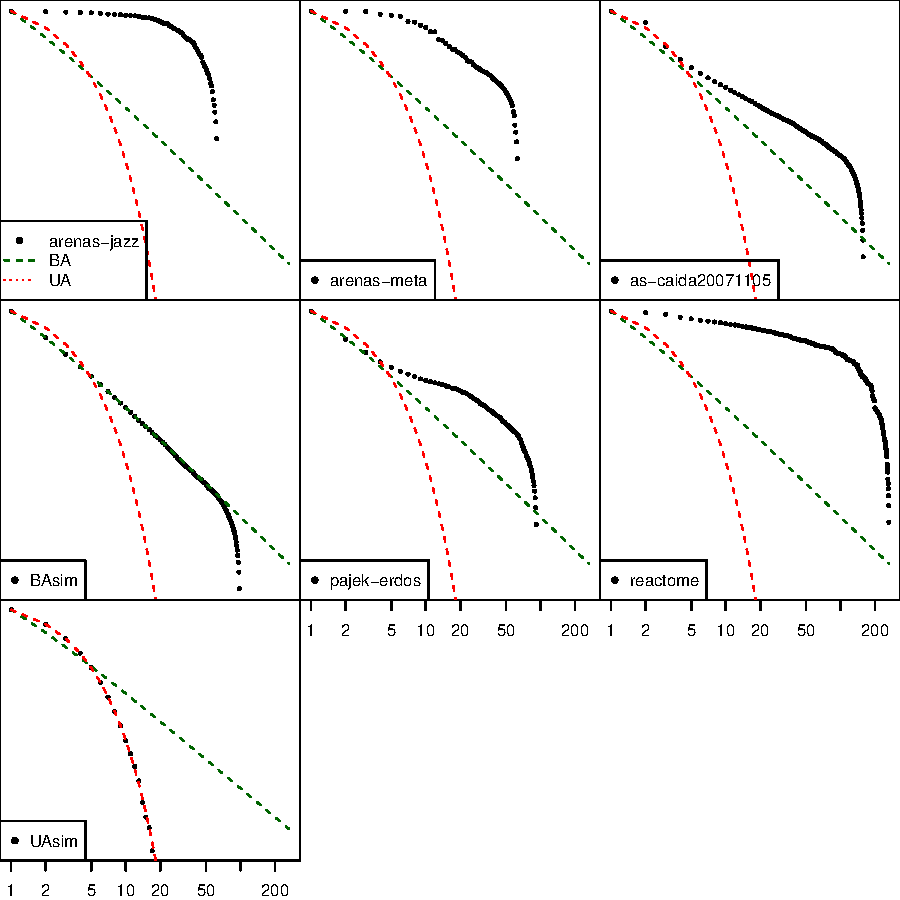
\includegraphics[width=0.66\textwidth,height=\textheight]{doc_files/figure-pdf/fig-survs-1.pdf}

}

\caption{\label{fig-survs}Plots of survival functions of real networks
degrees, along with the degree distribution for the UA and the BA
models}

\end{figure}

Figure~\ref{fig-survs} shows the survival function of the degrees of
various real networks as well as ``BA Simulated'' and ``UA Simulated''
which were generated using the corresponding schemes in
Section~\ref{sec-gen}. Additionally, the theoretical limiting degree
distribution of both the UA model and the BA model (for m=1) are
included on the plots. Visually it seems that neither of these models
are adequate for modelling the growth of the real networks shown here.

To further investigate this, Section~\ref{sec-realmodel} considers
fitting a model to these data that will provide insight into what would
be needed from a network generative model such that it flexible enough
to capture the variation of shapes of degree distribution in real
networks.

\hypertarget{sec-realmodel}{%
\section{Modelling degree distributions}\label{sec-realmodel}}

As mentioned in Section~\ref{sec-mod}, the method used here to model the
extreme values of the data will be a spliced threshold mixture.
Specifically, it will be a spliced threshold mixture of a power law and
a discretisation of the generalised Pareto distribution similar to what
is defined in {[}\protect\hyperlink{ref-Rohrbeck_2018}{16}{]}.

\begin{definition}[Power-Law IGP
Distribution]\protect\hypertarget{def-pligp}{}\label{def-pligp}

\[
f(y) = \begin{cases}
(1-\phi)\displaystyle\frac{y^{-(\alpha+1})}{\sum_{k=1}^v}k^{\alpha+1}, & y=1,2,\ldots, v\\
\phi\left[\left(1+\displaystyle\frac{\xi(y+1-v)}{\sigma_0+\xi v}\right)_+^{-1/\xi}-\left(1+\displaystyle\frac{\xi(y-v)}{\sigma_0+\xi v}\right)_+^{-1/\xi}\right],&y=v+1, v+2,\ldots
\end{cases}
\] where \(\alpha\in\mathbb R^+\) is the power law index and
\(\xi \in \mathbb R\) , \(\sigma_0 \in \mathbb R^+\) and
\(v\in\mathbb Z^+.\)

\end{definition}

\hypertarget{fitting-model-to-the-data}{%
\section{Fitting model to the data}\label{fitting-model-to-the-data}}

The values of the parameters in the model for each data set were
estimated under the Bayesian framework using a Metropolis within Gibbs
sampler. Below are plots showing the same data as in
Figure~\ref{fig-survs} but with the mean and 95\% credible intervals of
the survival function of the model for each data-set.

\begin{figure}[H]

{\centering 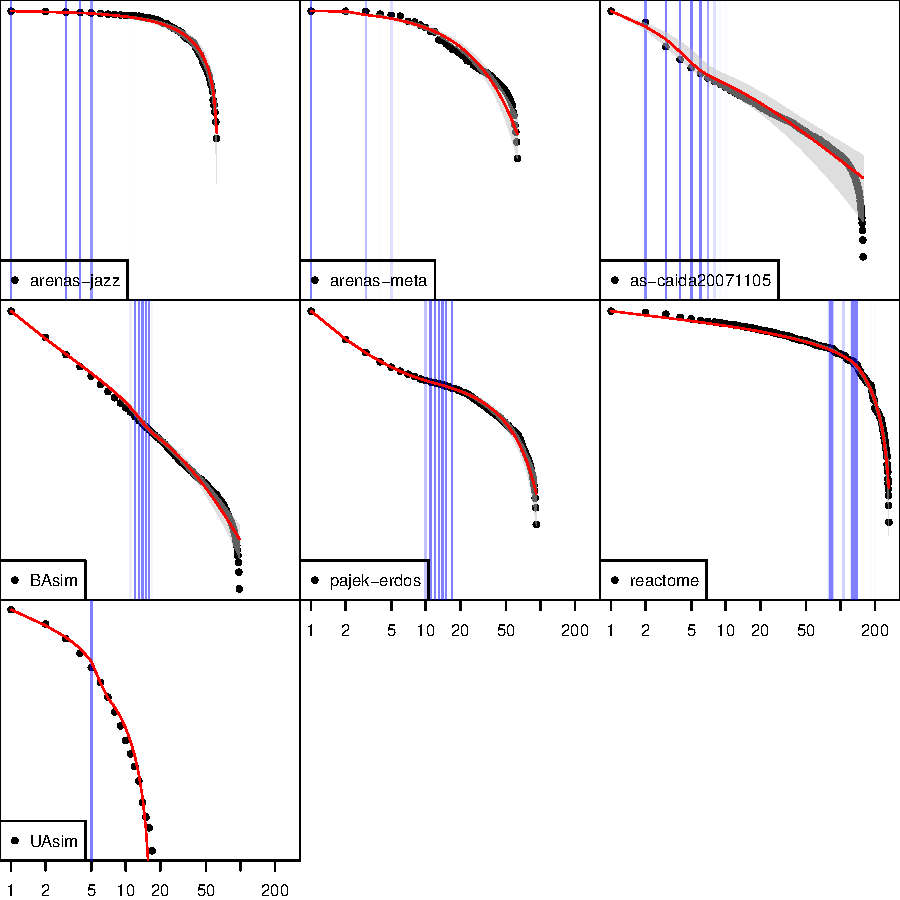
\includegraphics[width=0.66\textwidth,height=\textheight]{doc_files/figure-pdf/fig-fits1-1.pdf}

}

\caption{\label{fig-fits1}Survival functions from
Figure~\ref{fig-survs}, with mean and 95\% CI for the fitted model}

\end{figure}

As show by Figure~\ref{fig-fits1} the model seems to fit the data quite
well, below are some plot summarising each of the parameters for each of
the models:

\begin{figure}[H]

{\centering 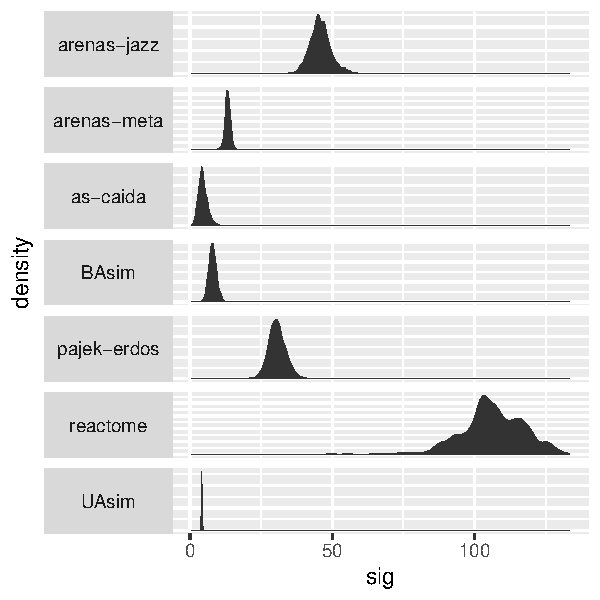
\includegraphics[width=0.66\textwidth,height=\textheight]{doc_files/figure-pdf/fig-scale-1.pdf}

}

\caption{\label{fig-scale}Posterior of scale (\(\sigma\))}

\end{figure}

\begin{figure}

\begin{minipage}[t]{0.50\linewidth}

{\centering 

\begin{figure}[H]

{\centering 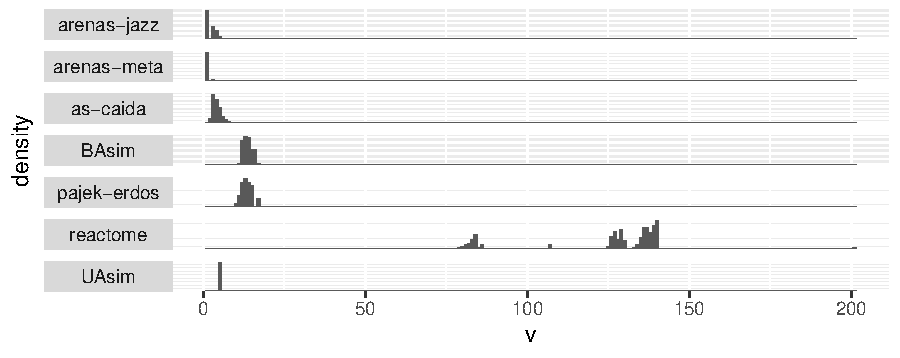
\includegraphics[width=1\textwidth,height=\textheight]{doc_files/figure-pdf/fig-thresh-1.pdf}

}

\caption{\label{fig-thresh}Posterior of threshold (\(v\))}

\end{figure}

}

\end{minipage}%
%
\begin{minipage}[t]{0.50\linewidth}

{\centering 

\begin{figure}[H]

{\centering 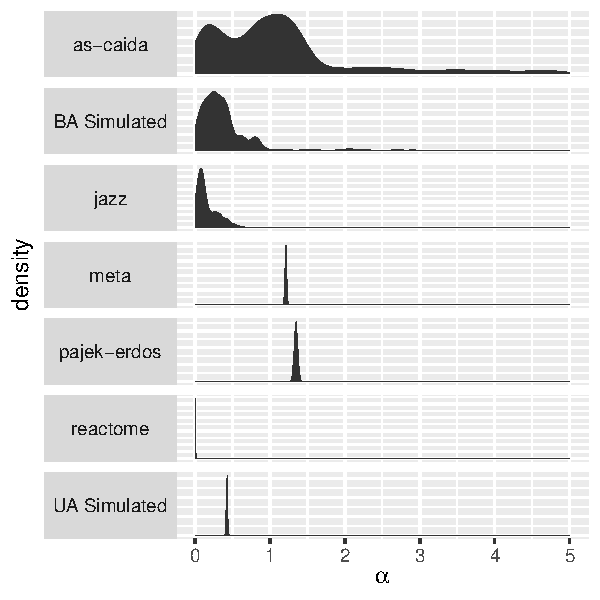
\includegraphics[width=1\textwidth,height=\textheight]{doc_files/figure-pdf/fig-alpha-1.pdf}

}

\caption{\label{fig-alpha}Posterior of power law index (\(\alpha\))}

\end{figure}

}

\end{minipage}%
\newline
\begin{minipage}[t]{0.50\linewidth}

{\centering 

\begin{figure}[H]

{\centering 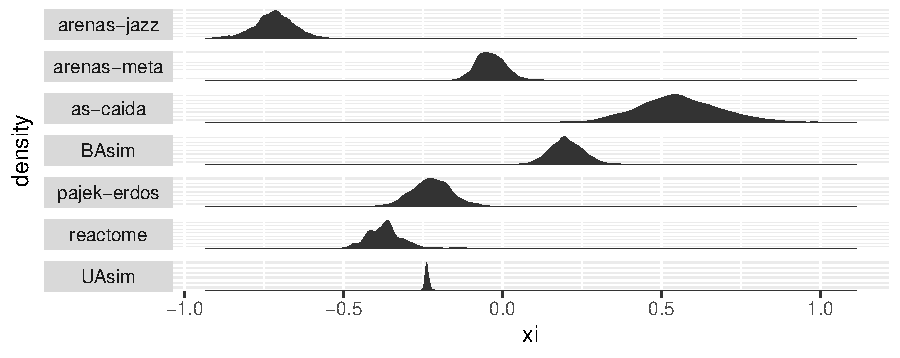
\includegraphics[width=1\textwidth,height=\textheight]{doc_files/figure-pdf/fig-shape-1.pdf}

}

\caption{\label{fig-shape}Posterior of shape (\(\xi\))}

\end{figure}

}

\end{minipage}%
%
\begin{minipage}[t]{0.50\linewidth}

{\centering 

\begin{figure}[H]

{\centering 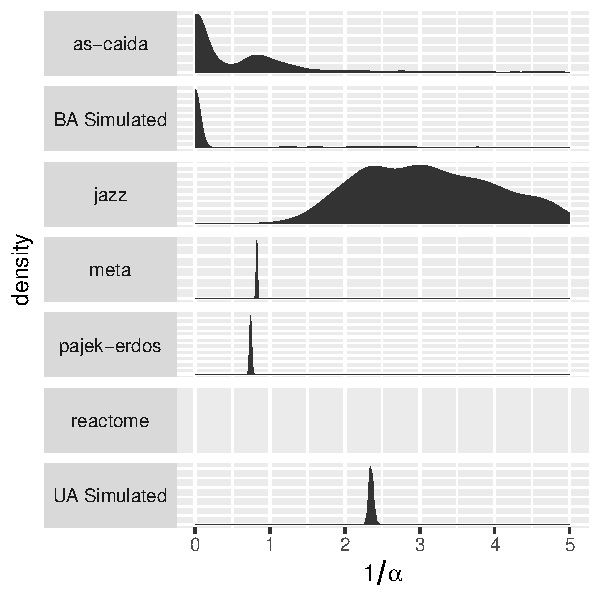
\includegraphics[width=1\textwidth,height=\textheight]{doc_files/figure-pdf/fig-alpha-inv-1.pdf}

}

\caption{\label{fig-alpha-inv}Posterior of inverse of power law index
(\(1/\alpha\))}

\end{figure}

}

\end{minipage}%

\end{figure}

Figure~\ref{fig-thresh} shows that for `arenas-meta' and `UAsim' the
posterior of the threshold is extremely concentrated, so much so that
only one threshold is used. In the case of `arenas-meta', this value is
1 meaning that the power law index \(\alpha\) (Figure~\ref{fig-alpha})
is free to be any value that is permitted by the prior, which is
anything on the positive real line, explaining the very diffuse
posterior. The threshold for `UAsim' is so low due to the magnitude of
the values in the data and is much more concentrated because of the
sample size.

The variety of values that \(\alpha\) and \(\xi\) take across all of the
data sets shown in Figure~\ref{fig-alpha} and Figure~\ref{fig-shape},
makes it clear that none of these models could have been the result of
either the BA model or the UA model when \(m=1\). Changing \(m\) may
indeed change the degree distribution, but it would also change the left
endpoint of the degree distributions as each vertex would join the graph
with \(m\) edges leaving no vertices with degree less that \(m\).

\hypertarget{general-preferential-attachment-analyses}{%
\section{General Preferential Attachment
Analyses}\label{general-preferential-attachment-analyses}}

So far it has been shown that neither the BA model nor the UA model can
adequately capture the range of type of degree distributions of real
networks. So, a natural place to start when attempting to expand the
range of possible degree distributions is the more general model, the
GPA. This section, will use results from
{[}\protect\hyperlink{ref-shimura12}{8}{]} and Section~\ref{sec-ext} to
investigate the possible types of degree distribution that may arise
from different preferential attachment functions in the GPA model.

\hypertarget{the-preferential-attachment-function}{%
\subsection{The Preferential Attachment
Function}\label{the-preferential-attachment-function}}

From here on the preferential functions that will be used for the GPA
model will be of the form: \[
g(k) = k^\gamma, \qquad \gamma>0.
\]

This allows for investigating the cases where the preferential
attachment function is sub-linear (\(\gamma<1\)) and when it is
super-linear (\(\gamma>1\)).

\hypertarget{section}{%
\subsection{}\label{section}}

As discussed in Section~\ref{sec-disc}, the limiting value of
\(\Omega(F,n)\) can give a lot of information about the behaviour of a
discrete distribution at extreme values. Below is a plot showing the
value of this quantity as \(n\) increases for various different values
of \(\gamma\).

\begin{figure}[H]

{\centering 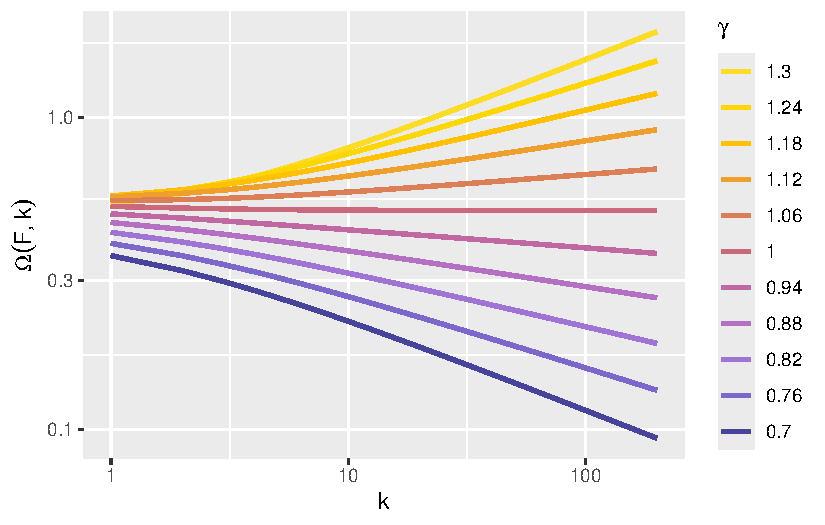
\includegraphics{doc_files/figure-pdf/fig-omega-1.pdf}

}

\caption{\label{fig-omega}Plot of \(\Omega(F,n)\) for various
\(\gamma \in (0.7,1.3)\)}

\end{figure}

Figure~\ref{fig-omega} shows that for \(\gamma<1\) \(\Omega(F,n)\) seems
to approach 0 as \(n\) increases, whereas for \(\gamma=1\)
\(\Omega(F,n)\) seems to converge to finite non-zero limit which is to
be expected as this corresponds to the BA model which has limiting
degree distribution in the Fréchet domain of attraction. However, for
\(\gamma>1\) the value of \(\Omega(F,n)\) appears to diverge and does
not approach a finite limit.

{[}\protect\hyperlink{ref-shimura12}{8}{]} does not provide any results
in particular for the case of \(\Omega(F,n)\) diverging but if the
definition of slow variation and thus super-heavy tails is viewed as
regular variation in the limit as \(\alpha\) goes to infinity then the
following can be obtained.

\begin{conjecture}[]\protect\hypertarget{cnj-omg}{}\label{cnj-omg}

For a distribution \(F\) with survival function \(\overline F\) and some
\(n\in\mathbb Z^+\), if: \[
\lim_{n\rightarrow\infty} \Omega(F,n) = \lim_{\alpha\downarrow0} \alpha^{-1} = \infty
\] then \(F\) has super heavy tails.

\end{conjecture}

This is further supported by Figure~\ref{fig-shtail} below, which shows
the value of the quantity from Definition~\ref{def-sup} for increasing
values of \(n\) and values of \(\gamma\) in the range \((1,2)\). The
plot shows the quantity approaching \(1\) for all values of \(\gamma\)
as \(n\) increases, suggesting that the limiting degree distribution of
the GPA model with \(g(k) = k^\gamma,\gamma>1\) has super heavy tails.

\begin{figure}[H]

{\centering 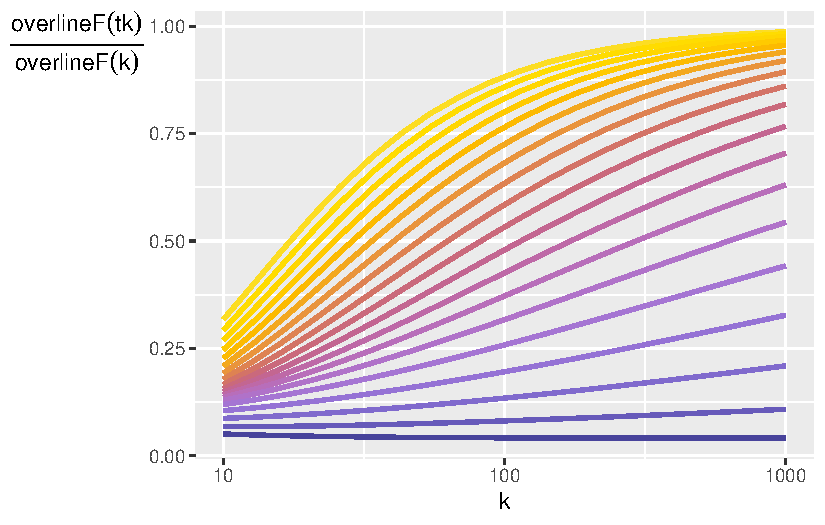
\includegraphics{doc_files/figure-pdf/fig-shtail-1.pdf}

}

\caption{\label{fig-shtail}Plot testing slow variation for
\(\gamma \in (1,2)\)}

\end{figure}

Figure~\ref{fig-shtail} is for \(t=5\), and the condition for super
heavy tails the quantity to approach one for all \(t>0\), other plots
were created for other values of \(t\) and changing \(t\) just changes
the rate of convergence to one.

\hypertarget{potential-novelty}{%
\section{Potential Novelty}\label{potential-novelty}}

The results from this subsection suggest that for super-linear
preferential attachment functions the GPA model has limiting degree
distribution with super heavy tails. This, along with results for the
linear case in Section~\ref{sec-gen} and sub-linear cases in
{[}\protect\hyperlink{ref-barabasibook}{15}{]} lead to the following
conjecture.

\begin{conjecture}[]\protect\hypertarget{cnj-gpa}{}\label{cnj-gpa}

The GPA model is only capable of producing three different types of
degree distribution:

\begin{enumerate}
\def\labelenumi{\arabic{enumi}.}
\tightlist
\item
  Gumbel: sub-linear preferential attachment function
  i.e.~\(g(k)=k^\gamma, \gamma\in(0,1)\)
\item
  Fréchet \(\mathcal D(\Phi_2)\): linear preferential attachment
  function i.e.~\(g(k)=k\)
\item
  Super heavy tails: super-linear preferential attachment function
  i.e.\(g(k)=k^\gamma, \gamma>1\)
\end{enumerate}

\end{conjecture}

This means that under the framework presented here, even the GPA model
is no where near close to being able to capture the range of types of
degree distribution found in real networks.

\hypertarget{discussion-and-next-steps}{%
\chapter{Discussion and Next Steps}\label{discussion-and-next-steps}}

The generative models considered so far are very simple, which is good
since the goal is to find as simple a model as possible. However, it is
clear now and perhaps unsurprising that the models shown here are not
capable of modelling realistic network growth. This section is dedicated
to discussing next steps for this project and address some questions
left open.

The models from Section~\ref{sec-gen} are very limited when it comes to
the actual growth of the network. Whenever a new vertex joins the
network it brings a fixed number of edges with it that remain
permanently, this is the only way that edges are added and thus the
degrees changed. Below are some modifications that could be made to
address this issue:

\begin{itemize}
\tightlist
\item
  Allow removal of edges throughout the networks growth.
\item
  Allow edges to be made between already existing vertices in the
  network.
\item
  Bring a random number of edges when a vertex is added.
\end{itemize}

It is possible to include all of these into a model with the
modification that at each time step you do one of three different steps
(Growth, Connection, Removal) with certain probabilities where the
number of edges added at each growth step is a discrete random variable.
Something similar could be done for the connection and removal steps.

Additionally, all of the models assume a constant preferential
attachment function both over time and across vertices. To address this
the preferential attachment function could be allowed to change over
time and perhaps differ between vertices. This would allow a vertex to
`age' in a sense, and could also allow for `categories' of vertices that
share the same preferential attachment function which differs from those
in other `categories'.

\appendix

\hypertarget{sec-plan}{%
\chapter{Updated Project Plan}\label{sec-plan}}

Progress so far is in line with the original project plan, so a lot of
this plan remains the same.

\hypertarget{objectives-and-more-specific-goals}{%
\section{Objectives and more specific
goals}\label{objectives-and-more-specific-goals}}

\hypertarget{continue-investigating-possible-modifications-to-barabuxe1si-albert-model-months-9-24}{%
\subsection*{Continue investigating possible modifications to
Barabási-Albert model (months
9-24)}\label{continue-investigating-possible-modifications-to-barabuxe1si-albert-model-months-9-24}}
\addcontentsline{toc}{subsection}{Continue investigating possible
modifications to Barabási-Albert model (months 9-24)}

So far, it has become clear that modifying the preferential attachment
function alone is not enough to make the BA model more suitable for real
networks. The next step is to investigate other possible modifications,
for example adding the ability to remove edge along with the possibility
of adding edges throughout the networks growth but not necessarily when
a new vertex is added, {[}\protect\hyperlink{ref-lu04}{17}{]} and
{[}\protect\hyperlink{ref-moore06}{18}{]} are possible starting points.

In addition to adding the possibility of edge removal, modifying the
preferential attachment function over time could also be possible.

\hypertarget{monitor-changes-in-model-parameters-of-various-real-networks-months-18-24}{%
\subsubsection*{Monitor changes in model parameters of various real
networks (months
18-24)}\label{monitor-changes-in-model-parameters-of-various-real-networks-months-18-24}}
\addcontentsline{toc}{subsubsection}{Monitor changes in model parameters
of various real networks (months 18-24)}

Fitting the model for degree distributions to real networks and
monitoring the changes in parameters over time will be an invaluable
resource when it comes time to develop modifications to the generative
model. This will be an ongoing process during some other steps but will
require a set of functions and/or an R package to be developed that can
efficiently estimate the parameters.

\hypertarget{use-these-changes-to-inform-the-possbile-modifications-months-24-30}{%
\subsubsection*{Use these changes to inform the possbile modifications
(months
24-30)}\label{use-these-changes-to-inform-the-possbile-modifications-months-24-30}}
\addcontentsline{toc}{subsubsection}{Use these changes to inform the
possbile modifications (months 24-30)}

As modifications are made to the generative model, the changes in model
parameters over time can also be recorded for the modified generative
models to make sure that they align with real networks.

\hypertarget{investigate-properties-of-the-new-model-months-30-36}{%
\subsubsection*{Investigate properties of the new model (months
30-36)}\label{investigate-properties-of-the-new-model-months-30-36}}
\addcontentsline{toc}{subsubsection}{Investigate properties of the new
model (months 30-36)}

Once a set of modifications has been developed, the theoretical
properties of networks that grow under the new model will be important
to study.

\hypertarget{outcomes}{%
\section{Outcomes}\label{outcomes}}

\hypertarget{validate-current-model-for-degree-distribution-is-suitable-month-12}{%
\subsubsection*{Validate current model for degree distribution is
suitable (\textasciitilde month
12)}\label{validate-current-model-for-degree-distribution-is-suitable-month-12}}
\addcontentsline{toc}{subsubsection}{Validate current model for degree
distribution is suitable (\textasciitilde month 12)}

The current model seems to perform fairly well when fitting to real
networks, but a more robust method for testing how well the model fits
could be used to make sure that it is suitable. There are perhaps some
indications that a third component should be added to the spliced
mixture model.

\hypertarget{create-set-of-functions-to-fit-the-model-month-18}{%
\subsubsection*{Create set of functions to fit the model
(\textasciitilde month
18)}\label{create-set-of-functions-to-fit-the-model-month-18}}
\addcontentsline{toc}{subsubsection}{Create set of functions to fit the
model (\textasciitilde month 18)}

Once a suitable model for the degree distribution has been decided on,
an efficient and fairly uninvolved way to fit the model needs to be
developed. This is to aid with monitoring changes in parameters over
time, as it will need to be fitted to many sets of data over many time
frames.

\hypertarget{develop-modifiations-of-the-barabuxe1si-albert-model-month-30}{%
\subsubsection*{Develop modifiations of the Barabási-Albert model
(\textasciitilde month
30)}\label{develop-modifiations-of-the-barabuxe1si-albert-model-month-30}}
\addcontentsline{toc}{subsubsection}{Develop modifiations of the
Barabási-Albert model (\textasciitilde month 30)}

A new model will be developed based on modifications of the
Barabási-Albert model that can more accurately describe how real
networks have grown.

\hypertarget{training}{%
\chapter{Training}\label{training}}

\hypertarget{school-training}{%
\section{School Training}\label{school-training}}

I attended two weeks of APTS courses, one in Warwick which included two
modules on Statistical Computing and Statistical Inference, and another
in Nottingham which included modules on Applied Stochastic Processes and
Statistical Modelling.

\hypertarget{conferences}{%
\section{Conferences}\label{conferences}}

I attended one conference this year, the SAgE PGR conference where I
presented a poster summarising the work I had done up until that point.

\hypertarget{training-still-required}{%
\section{Training still required}\label{training-still-required}}

There is still some training I still need to do:

\begin{itemize}
\tightlist
\item
  c++ training.
\item
  Training on Rocket HPC.
\end{itemize}

\hypertarget{funding-and-stipend}{%
\section*{Funding and Stipend}\label{funding-and-stipend}}
\addcontentsline{toc}{section}{Funding and Stipend}

The funding for this project expires on \textbf{17th March 2027}.

\hypertarget{references}{%
\chapter*{References}\label{references}}
\addcontentsline{toc}{chapter}{References}

\hypertarget{refs}{}
\begin{CSLReferences}{0}{0}
\leavevmode\vadjust pre{\hypertarget{ref-caida}{}}%
\CSLLeftMargin{1. }%
\CSLRightInline{(2017)
\href{http://konect.cc/networks/as-caida20071105}{CAIDA network dataset
-- {KONECT}}}

\leavevmode\vadjust pre{\hypertarget{ref-jazz}{}}%
\CSLLeftMargin{2. }%
\CSLRightInline{(2017) \href{http://konect.cc/networks/arenas-jazz}{Jazz
musicians network dataset -- {KONECT}}}

\leavevmode\vadjust pre{\hypertarget{ref-meta}{}}%
\CSLLeftMargin{3. }%
\CSLRightInline{(2017)
\href{http://konect.cc/networks/arenas-meta}{Caenorhabditis elegans
network dataset -- {KONECT}}}

\leavevmode\vadjust pre{\hypertarget{ref-pajek}{}}%
\CSLLeftMargin{4. }%
\CSLRightInline{(2018)
\href{http://konect.cc/networks/pajek-erdos}{Erdős network dataset --
{KONECT}}}

\leavevmode\vadjust pre{\hypertarget{ref-reactome}{}}%
\CSLLeftMargin{5. }%
\CSLRightInline{(2017)
\href{http://konect.cc/networks/reactome}{Reactome network dataset --
{KONECT}}}

\leavevmode\vadjust pre{\hypertarget{ref-haan06}{}}%
\CSLLeftMargin{6. }%
\CSLRightInline{Haan L, Ferreira A (2006)
\href{https://doi.org/10.1007/0-387-34471-3}{Extreme value theory: An
introduction}}

\leavevmode\vadjust pre{\hypertarget{ref-fmh09}{}}%
\CSLLeftMargin{7. }%
\CSLRightInline{Fraga Alves M, Haan L, Neves C (2009) A test procedure
for detecting super-heavy tails. Journal of Statistical Planning and
Inference 139. \url{https://doi.org/10.1016/j.jspi.2008.04.026}}

\leavevmode\vadjust pre{\hypertarget{ref-shimura12}{}}%
\CSLLeftMargin{8. }%
\CSLRightInline{Shimura T (2012) Discretization of distributions in the
maximum domain of attraction. Extremes 15:299--317.
\url{https://doi.org/10.1007/s10687-011-0137-7}}

\leavevmode\vadjust pre{\hypertarget{ref-hds24}{}}%
\CSLLeftMargin{9. }%
\CSLRightInline{Hitz AS, Davis RA, Samorodnitsky G (2024) Discrete
extremes. Journal of Data Science 1--13.
\url{https://doi.org/10.6339/24-JDS1120}}

\leavevmode\vadjust pre{\hypertarget{ref-agn22}{}}%
\CSLLeftMargin{10. }%
\CSLRightInline{Ahmad T, Gaetan C, Naveau P (2022)
\href{https://arxiv.org/abs/2210.15253}{Modelling of discrete extremes
through extended versions of discrete generalized pareto distribution}.
ArXiv e-prints}

\leavevmode\vadjust pre{\hypertarget{ref-coles2001}{}}%
\CSLLeftMargin{11. }%
\CSLRightInline{Coles S (2001)
\href{https://books.google.co.uk/books?id=2nugUEaKqFEC}{An introduction
to statistical modeling of extreme values}. Springer}

\leavevmode\vadjust pre{\hypertarget{ref-mac2012}{}}%
\CSLLeftMargin{12. }%
\CSLRightInline{Scarrott C, MacDonald A (2012) A review of extreme value
threshold estimation and uncertainty quantification. Revstat Statistical
Journal 10:33--60. \url{https://doi.org/10.57805/revstat.v10i1.110}}

\leavevmode\vadjust pre{\hypertarget{ref-rudas07}{}}%
\CSLLeftMargin{13. }%
\CSLRightInline{Rudas A, Tóth B, Valkó B (2007) Random trees and general
branching processes. Random Structures \& Algorithms 31(2):186--202.
https://doi.org/\url{https://doi.org/10.1002/rsa.20137}}

\leavevmode\vadjust pre{\hypertarget{ref-Barabasi99}{}}%
\CSLLeftMargin{14. }%
\CSLRightInline{Barabási A-L, Albert R (1999) Emergence of scaling in
random networks. Science 286(5439):509--512.
\url{https://doi.org/10.1126/science.286.5439.509}}

\leavevmode\vadjust pre{\hypertarget{ref-barabasibook}{}}%
\CSLLeftMargin{15. }%
\CSLRightInline{Barabási AL, PÃ3sfai MÃ (2016)
\href{https://books.google.co.uk/books?id=iLtGDQAAQBAJ}{Network
science}. Cambridge University Press}

\leavevmode\vadjust pre{\hypertarget{ref-Rohrbeck_2018}{}}%
\CSLLeftMargin{16. }%
\CSLRightInline{Rohrbeck C, Eastoe EF, Frigessi A, Tawn JA (2018)
{Extreme value modelling of water-related insurance claims}. The Annals
of Applied Statistics 12(1):246--282.
\url{https://doi.org/10.1214/17-AOAS1081}}

\leavevmode\vadjust pre{\hypertarget{ref-lu04}{}}%
\CSLLeftMargin{17. }%
\CSLRightInline{Lu L, Chung F (2004) Coupling online and offline
analyses for random power law graphs. Internet Mathematics 1(4).
\url{https://doi.org/10.1080/15427951.2004.10129094}}

\leavevmode\vadjust pre{\hypertarget{ref-moore06}{}}%
\CSLLeftMargin{18. }%
\CSLRightInline{Moore C, Ghoshal G, Newman M (2006) Exact solutions for
models of evolving networks with addition and deletion of nodes.
Physical review E, Statistical, nonlinear, and soft matter physics
74:036121. \url{https://doi.org/10.1103/PhysRevE.74.036121}}

\end{CSLReferences}



\end{document}
